% gjilguid2e.tex
% V2.0 released 1998 December 18
% V2.1 released 2003 October 7 -- Gregor Hutton, updated the web address for the style files.

%\documentclass[extra,mreferee]{gji}
%\documentclass[extra, onecolumn, doublespacing]{gji}
%\documentclass[extra]{gji}
%\RequirePackage{lineno}
\documentclass[12pt,double]{article}


%\bibliographystyle{agufull08} % Uncomment when generating bibliography
%\usepackage{timet}
\usepackage[dvips]{graphicx}
\usepackage{amssymb}
\usepackage{amsmath}
\usepackage{rotating}
\usepackage{natbib}
\usepackage{lineno}
%\usepackage{titlesec}
\linenumbers

\linespread{1.5}

\newcommand{\mitbf}[1]{  
  \hbox{\mathversion{bold}$#1$}}  
  \newcommand{\rmn}[1] {{\mathrm #1}}  
  \newcommand{\itl}[1] {{\mathit #1}}  
  \newcommand{\bld}[1] {{\mathbf #1}}  


%\titleformat{\section}
%{\bf}{\thesection}{1em}{\MakeUppercase{#1}}

%\date{Received 2012 Month Day; in original form 2012 Month Day}
%\pagerange{\pageref{firstpage}--\pageref{lastpage}}
%\volume{200}
%\pubyear{2012}

%\def\LaTeX{L\kern-.36em\raise.3ex\hbox{{\small A}}\kern-.15em
%    T\kern-.1667em\lower.7ex\hbox{E}\kern-.125emX}
%\def\LATeX{L\kern-.36em\raise.3ex\hbox{{\Large A}}\kern-.15em
%    T\kern-.1667em\lower.7ex\hbox{E}\kern-.125emX}
% Authors with AMS fonts and mssymb.tex can comment out the following
% line to get the correct symbol for Geophysical Journal International.
\let\leqslant=\leq

\newtheorem{theorem}{Theorem}[section]

\begin{document}

%%=======================================================================================

%Figure 1
\begin{figure}
%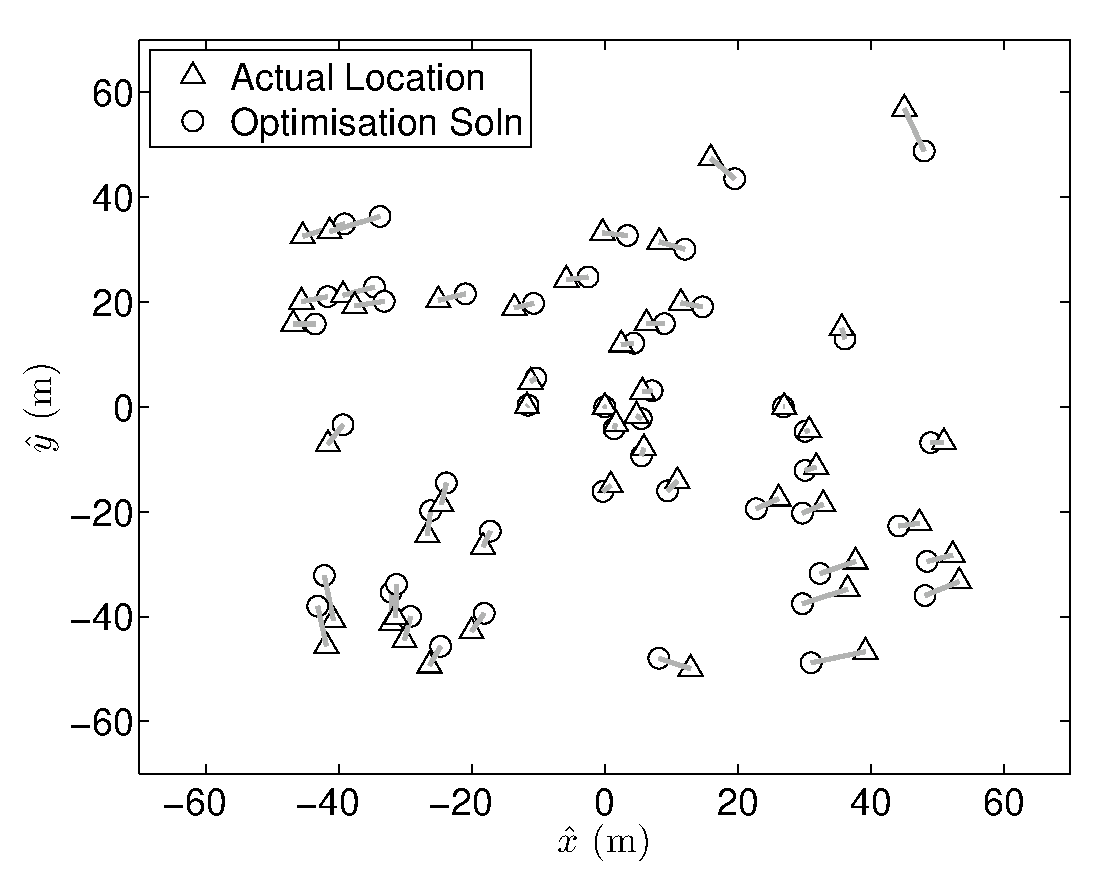
\includegraphics[width = 20pc]{diags/locs_2D_50eq_1.eps}
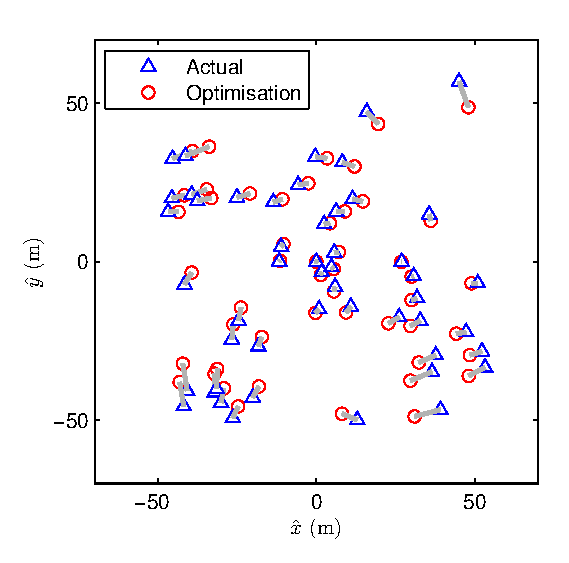
\includegraphics[width = 20pc]{Figure1_c.eps}
\caption{Example 1 - Synthetic relocation of 50 earthquakes in 2D
using all constraints with noise $\bar{\sigma}_N=0.02$. Actual and
optimization event locations are identified by triangles and circles,
respectively.} \label{fig-2D50eq-relocation_eg1}
\end{figure}

%%=======================================================================================

%Figure 2
\begin{figure}
%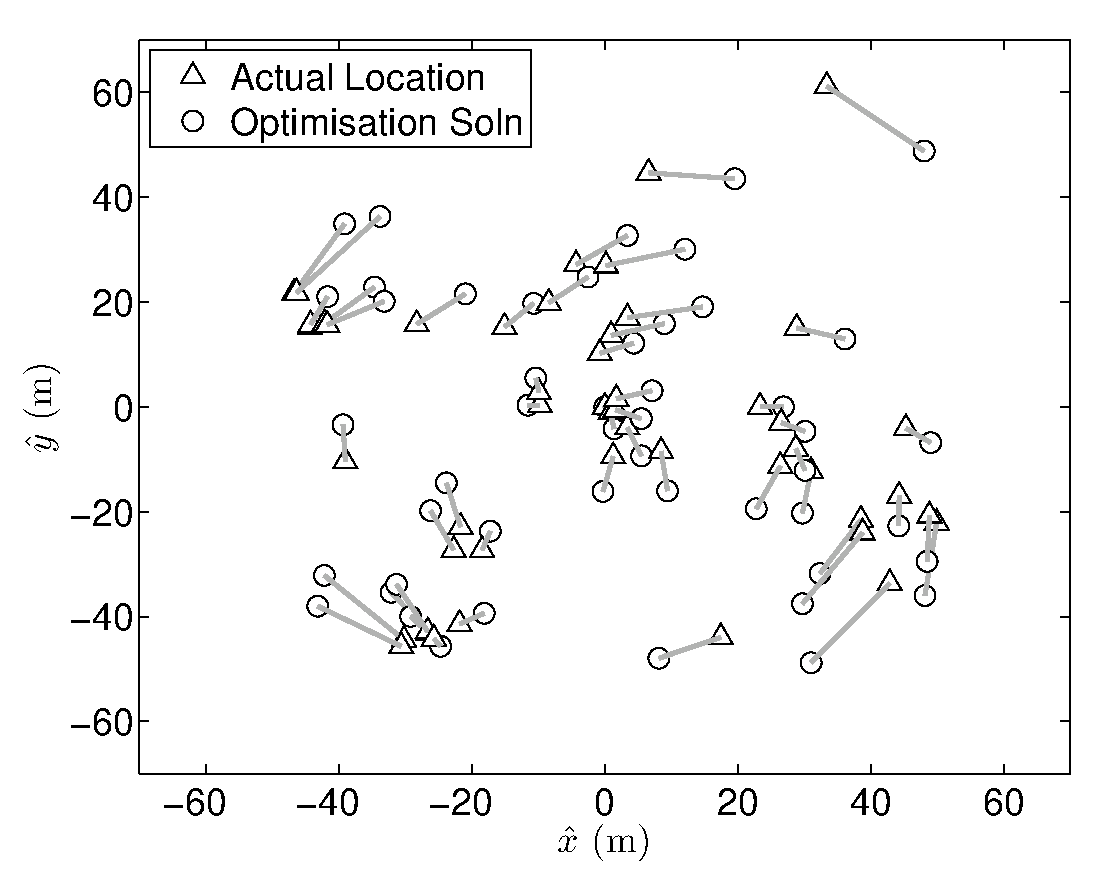
\includegraphics[width = 20pc]{diags/locs_2D_50eq_3.eps}
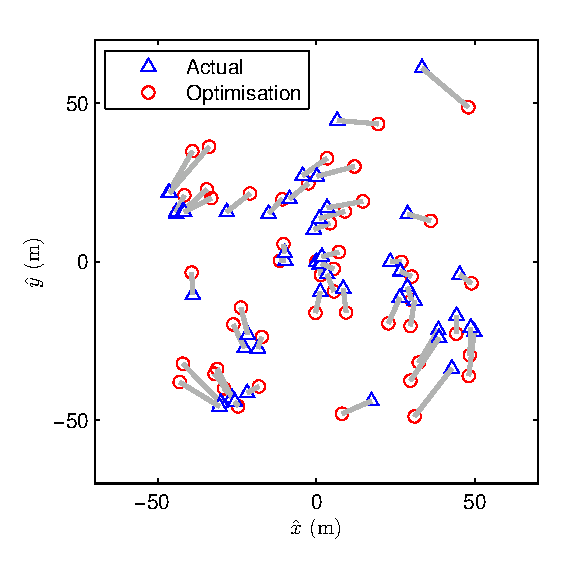
\includegraphics[width = 20pc]{Figure2_c.eps}
\caption{Example 2 - Synthetic relocation of 50 earthquakes in 2D
using all constraints with noise $\bar{\sigma}_N= 2
\epsilon(\delta_t)$.
 Actual and optimization event locations
are identified by triangles and circles, respectively.}
\label{fig-2D50eq-relocation_eg3}
\end{figure}

%%=======================================================================================

% Figure 3
\begin{figure}
%\noindent\includegraphics[width = 20pc]{../../thesis_version2/diags/eq_location_optimisation/synth2Dmulti/ressummary_2Dsynth50eq.eps}
%\noindent\includegraphics[width=20pc]{diags/synth2Dmulti/ressummary_2Dsynth50eq.eps}
\noindent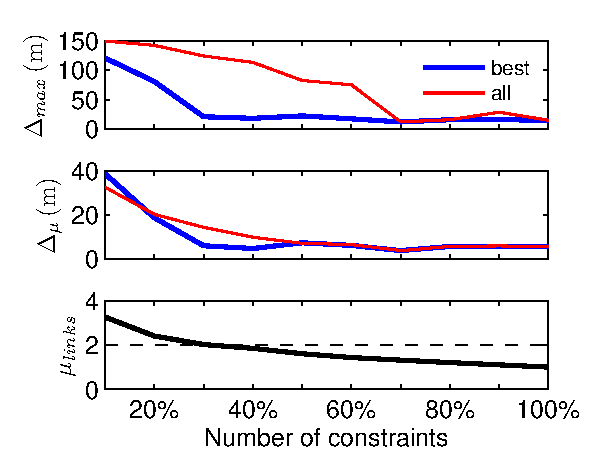
\includegraphics[width=20pc]{Figure3_c.eps}
\caption{Example 3 - Statistical measures of error in the
 solutions for the 2D synthetic cases when all and best
optimization results are considered. The statistics $\Delta_{max}$
and $\Delta_\mu$  are the maximum and mean coordinate error,
respectively. The bottom subplot shows the average minimum number of
branches required to link the 2450 pairs.}
 \label{fig:optimisationresults-2Dsynth}
\end{figure}

%%=======================================================================================

% Figure 4
\begin{figure}
%\noindent\includegraphics[width = 20pc]{../../thesis_version2/diags/eq_location_optimisation/synth3Dmulti/ressummary_3Dsynth50eq.eps}
%\noindent\includegraphics[width=20pc]{diags/synth3Dmulti/ressummary_3Dsynth50eq.eps}
\noindent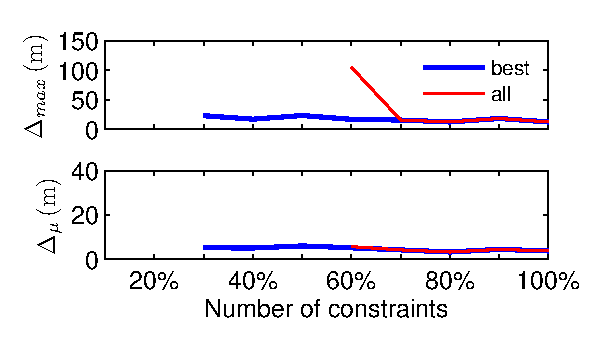
\includegraphics[width=20pc]{Figure4_c.eps}
\caption{Example 4 - Statistical measures of error in the
optimization solutions for the 3D synthetic cases when all
and best results are considered. The statistics
$\Delta_{max}$ and $\Delta_\mu$ are the maximum and mean coordinate
error, respectively. The absence of the lines below
60\% and 30\% indicates a breakdown in the solutions when all or
best optimization result(s) are considered, respectively.}
\label{fig:optimisationresults-3Dsynth}
\end{figure}

%%=======================================================================================

% Figure 5
\begin{figure}
%\noindent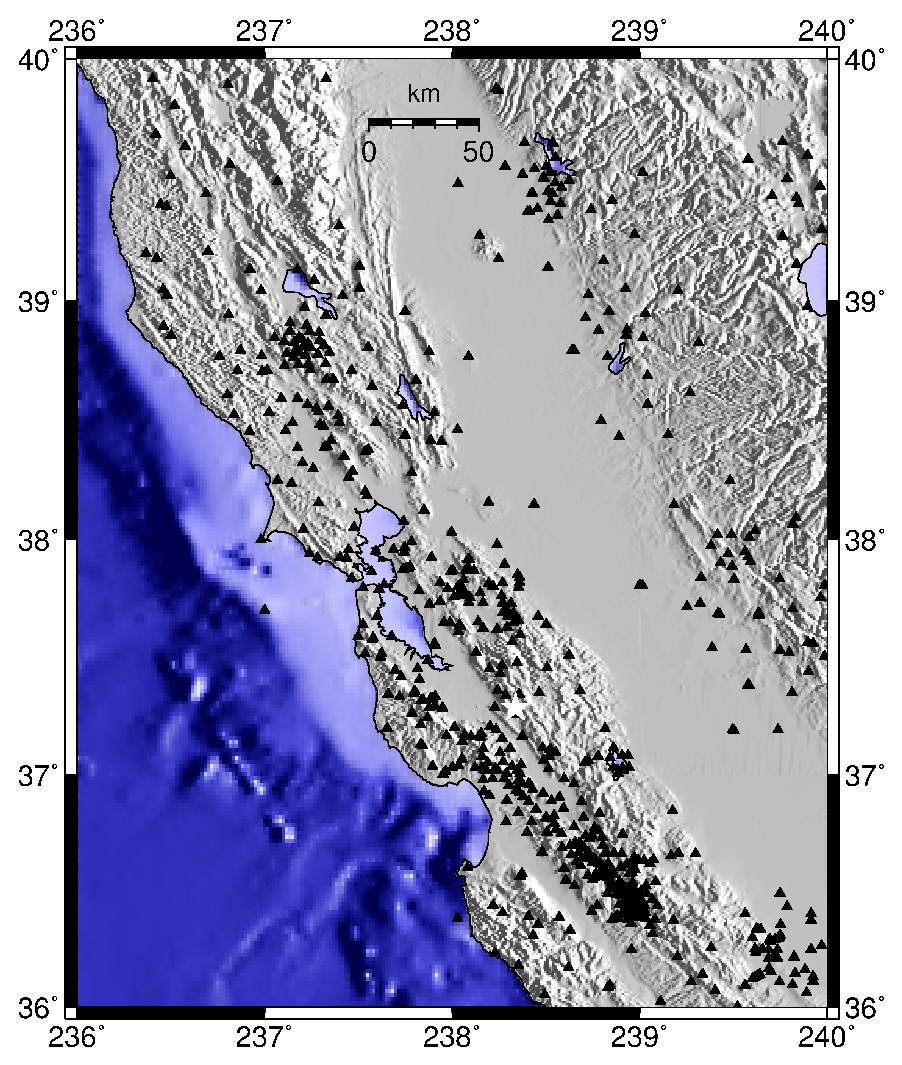
\includegraphics[width=20pc]{diags/CalaverasMap/gmt_california/CaliforniaCalaverasMap1.eps}
\noindent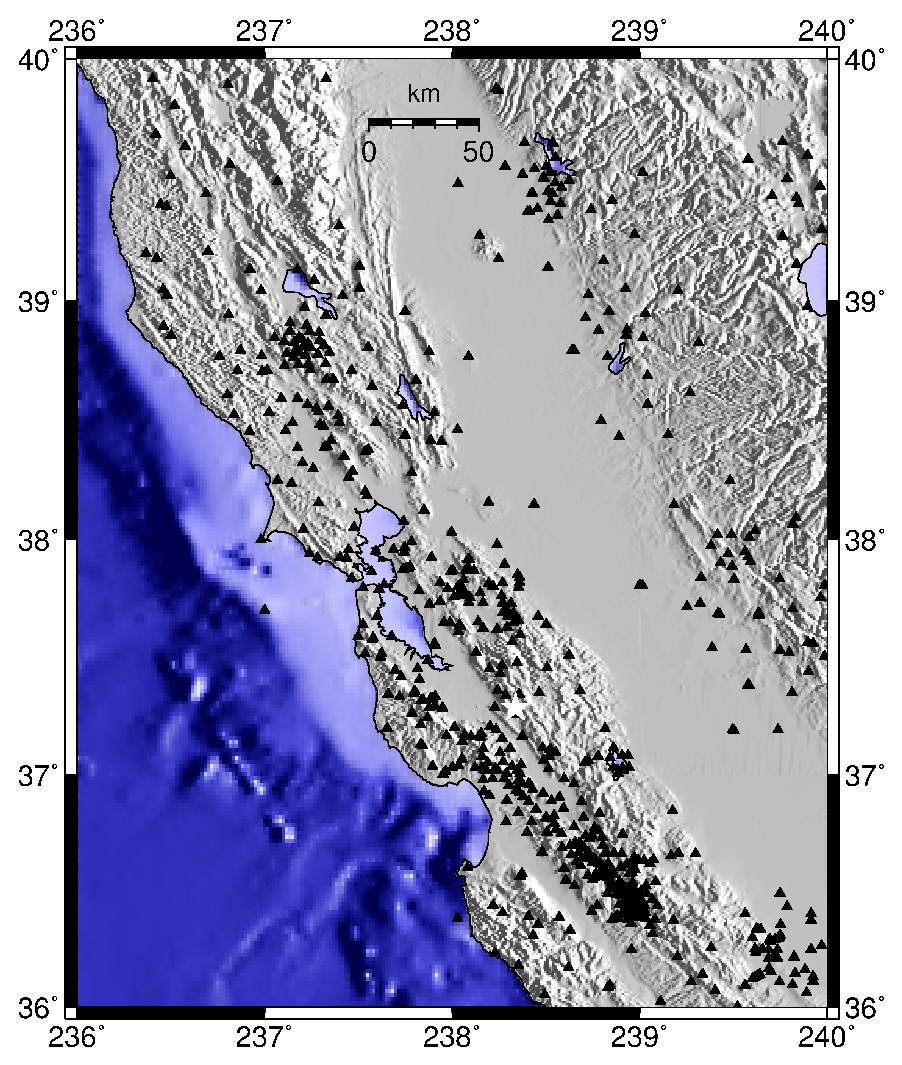
\includegraphics[width=20pc]{Figure5.eps} 
\caption{Map
showing location of the Calaveras cluster (star) and 805
seismic stations (triangles).}
\label{fig:-eqopti-California-Calaveras}
\end{figure}

%%=======================================================================================
% Figure 6

% Now we have the SVD version
\begin{figure}
%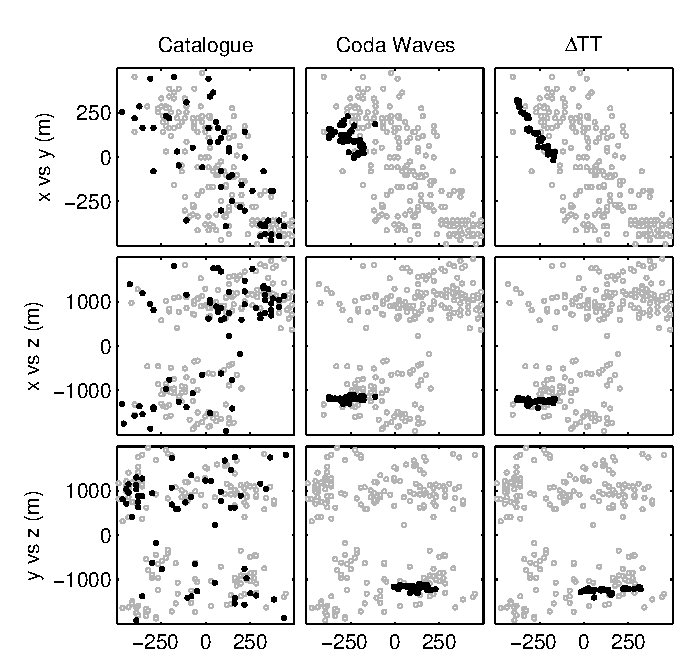
\includegraphics{diags/CalaverasLoc1_hypoDD_SVD.eps}
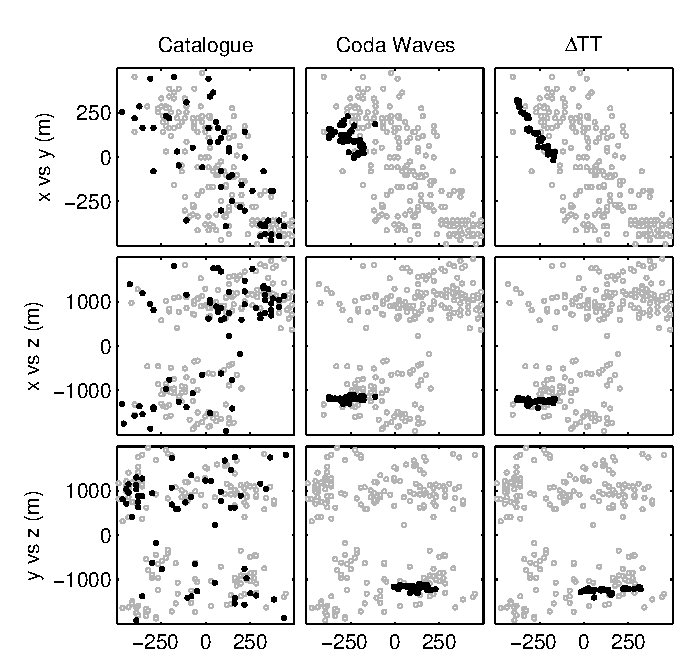
\includegraphics{Figure6_bw.eps}
\caption{Example 5 - Comparison of relative earthquake locations
using three different methods: catalogue location (column 1), CWI
(column 2) and hypoDD (column 3). Note that in the case of the
hypoDD and CWI inversions we consider only the 68 earthquakes in
black, the gray catalogue locations for the remaining 240 (308-68)
earthquakes are shown for the purpose of orientation only. In this and subsequent
similar figures (Figures \ref{fig-CWIreducesstats}, \ref{fig-HYPODDreducesstats},
\ref{fig-68Calaverasevents_ttandcoda1} and \ref{fig-68Calaverasevents_ttsubsetandcoda1}) 
$x$ is defined as positive towards the east, y is positive towards the north and z is 
positive down.}
\label{fig-69Calaverasevents_eg1}
\end{figure}
%%=======================================================================================

% Figure 7
\begin{figure}
%\noindent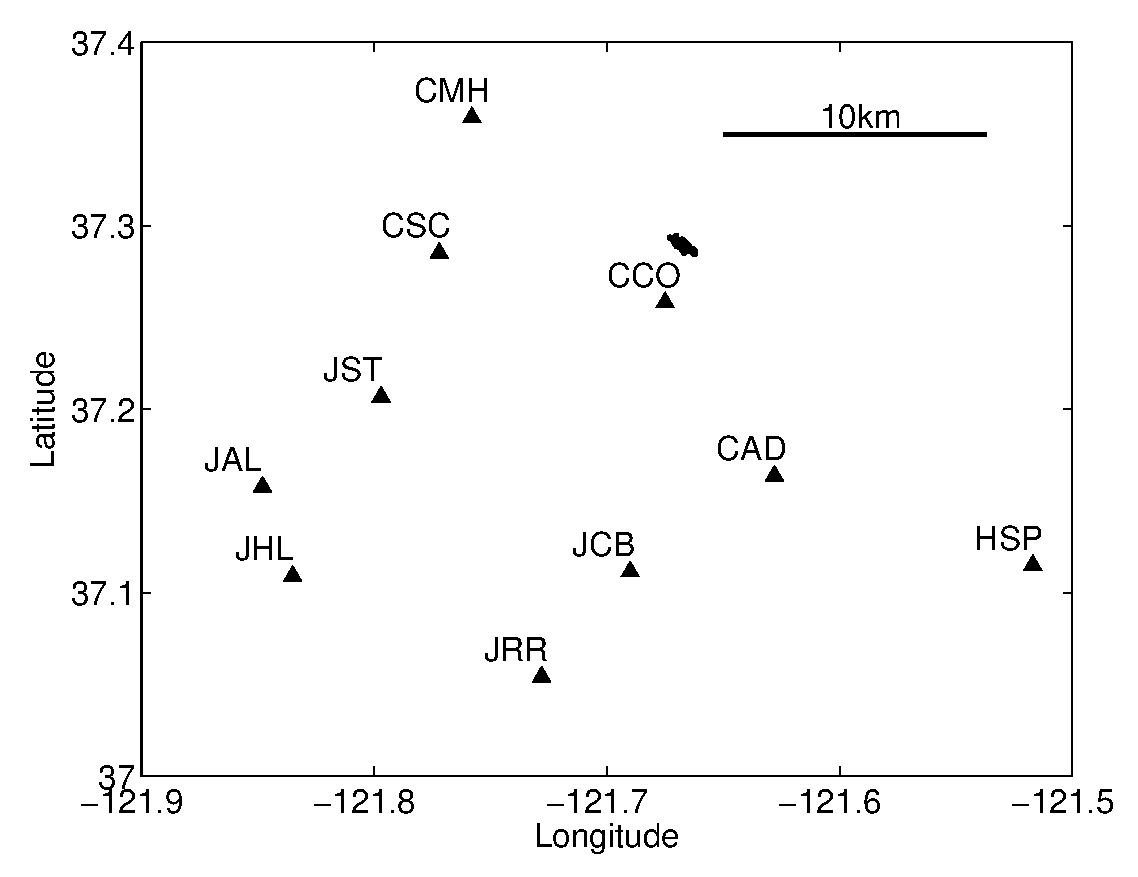
\includegraphics[width=20pc]{diags/CalaverasMap/matlab/Calaveras_substationmap}
\noindent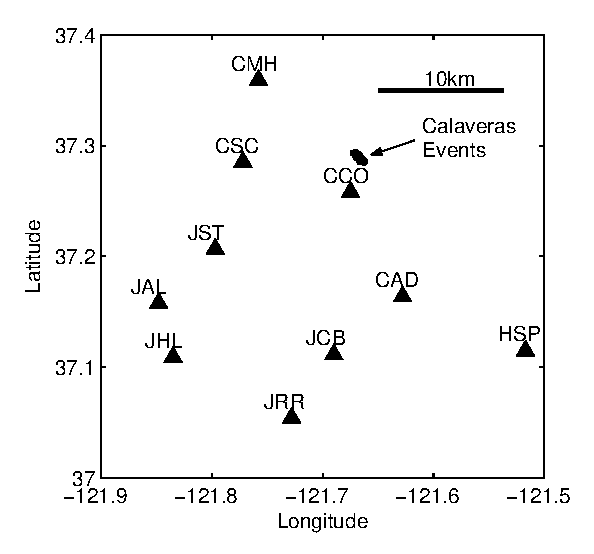
\includegraphics[width=20pc]{Figure7.eps} 
\caption{Location
of the 10 stations (triangles) used to relocate the Calaveras events
in Examples 6 to 8. Stations are removed one at a time according to
the order defined by the bracketed numbers. That is, JRR is the first station to 
be removed, JHL is the second and so on. Events are indicated with circles.}
\label{fig:-eqopti-Calaveras-substations}
\end{figure}

%%=======================================================================================

%Figure 8
\begin{figure}
%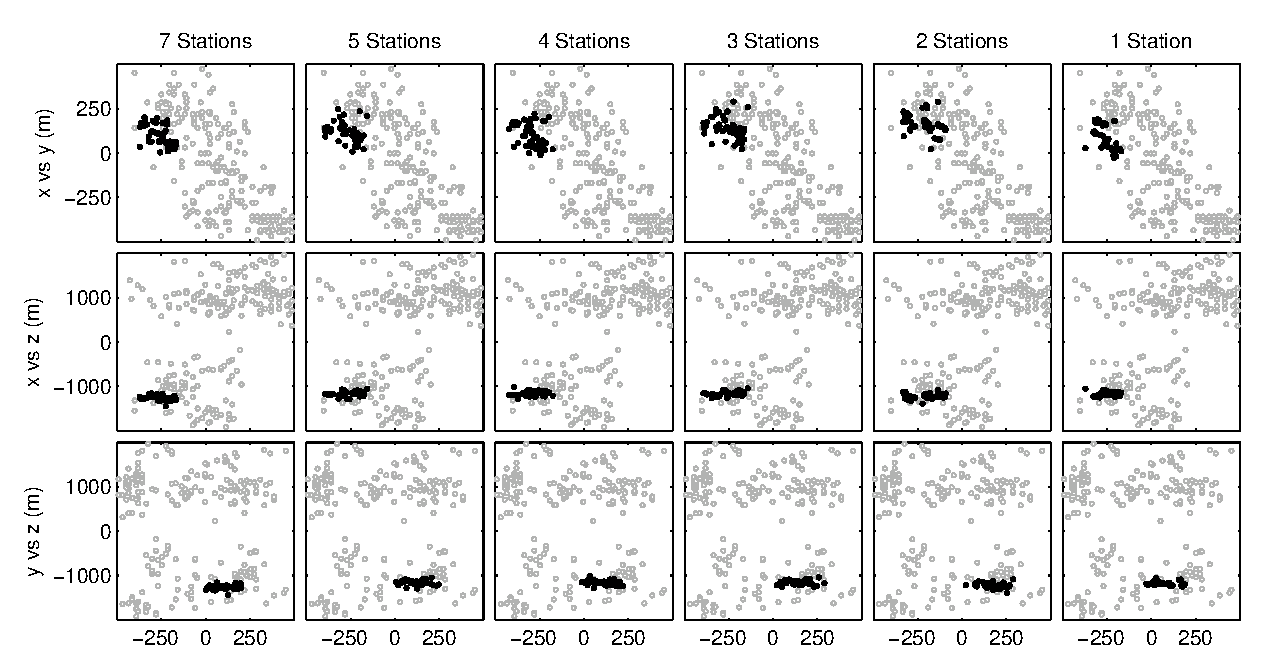
\includegraphics[angle=90,height = 50pc]{diags/CalaverasLoc2.eps}
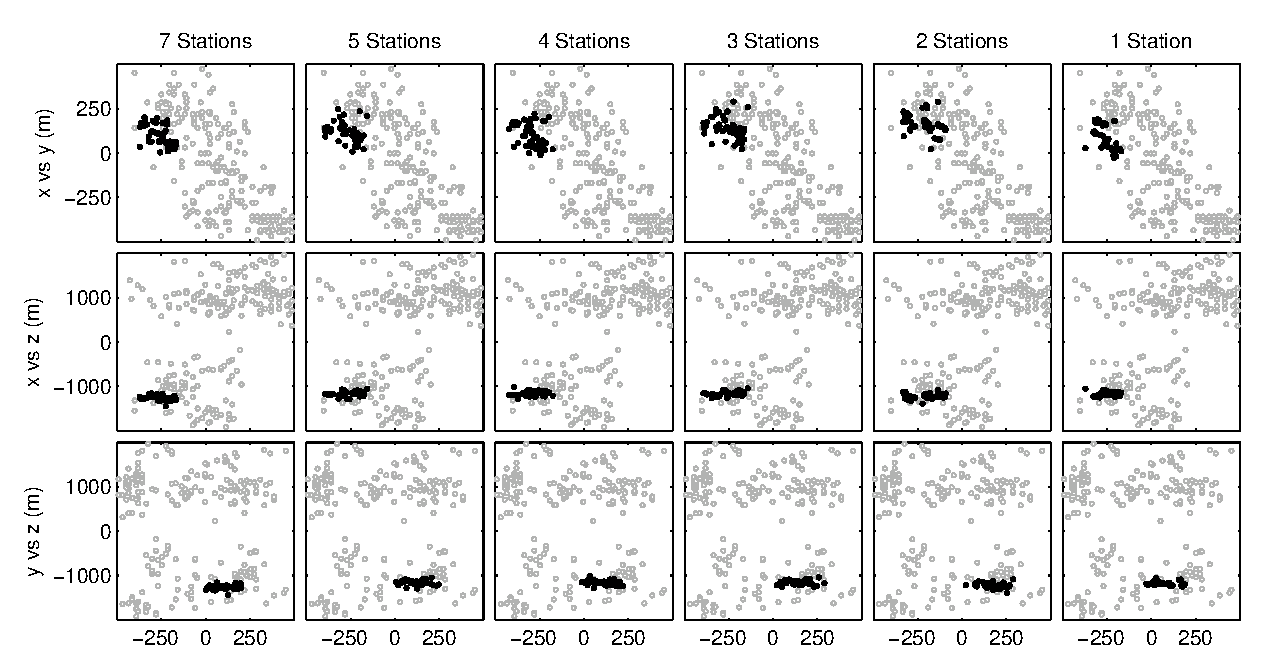
\includegraphics[angle=90,height = 50pc]{Figure8_bw.eps}
\caption{Example 6 - CWI relative locations with reduced stations. 
Axes as defined in Figure \ref{fig-69Calaverasevents_eg1}.
\hspace{20em}}
\label{fig-CWIreducesstats}
\end{figure}

%%=========================================================================
% Figure 9

% This is the version using hypoDD with SVD
\begin{figure}
%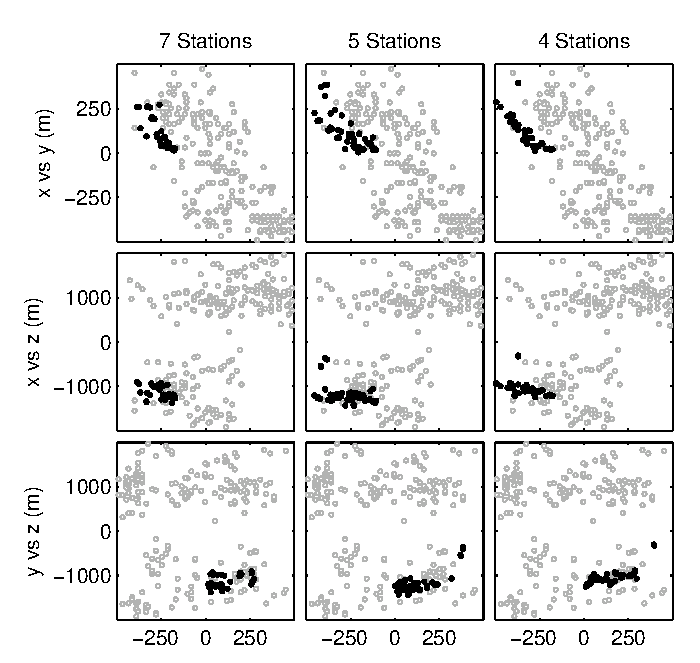
\includegraphics[height = 25pc]{diags/CalaverasLoc3_hypoDD_SVD.eps}
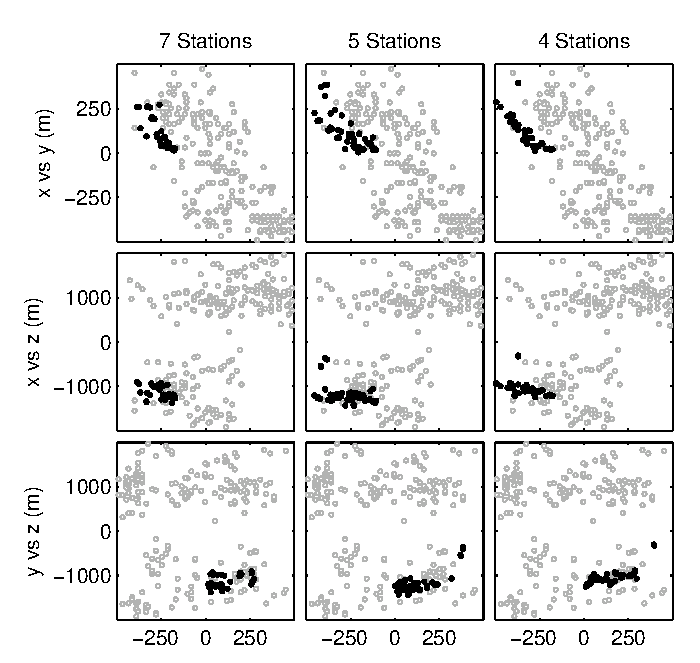
\includegraphics[height = 25pc]{Figure9_bw.eps}
\caption{Example 6 - HypoDD (SVD) relative locations with reduced
stations. Axes as defined in Figure \ref{fig-69Calaverasevents_eg1}. 
\hspace{20em} }
\label{fig-HYPODDreducesstats}
\end{figure}
%%=========================================================================

%Figure 10

% This is the version using hypoDD with SVD
\begin{figure}
%\noindent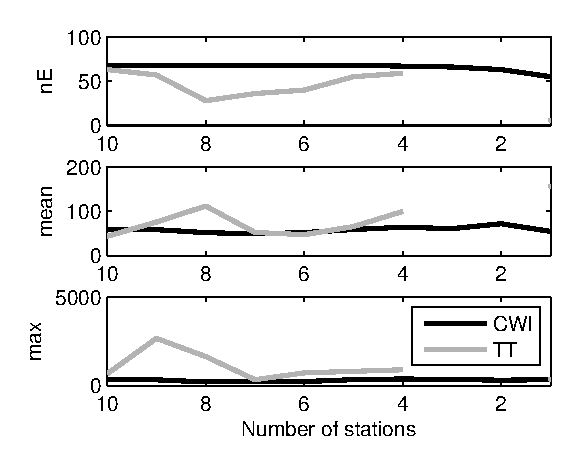
\includegraphics[width=20pc]{diags/CalaverasLoc4_hypoDD_SVD.eps}
\noindent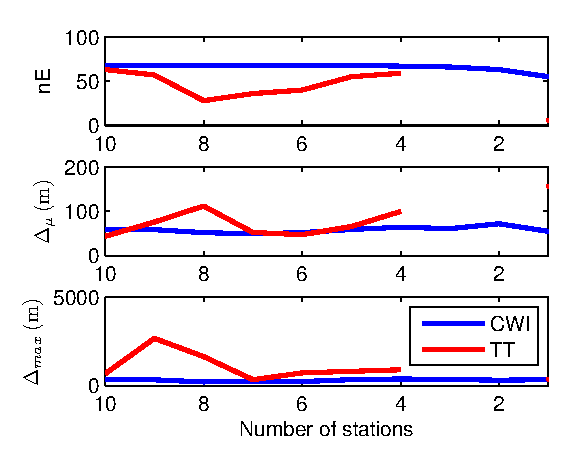
\includegraphics[width=20pc]{Figure10_c.eps}
\caption{Example 6 - Number of constrainable events $nE$ in the CWI
and hypoDD inversions as a function of the number of stations considered
(top). Mean (middle) and maximum (bottom) of the difference computed
between the reduced station inversion results (CWI and hypoDD) and
the complete hypoDD locations for all 308 events. }
\label{fig-statremoval_summarystats}
\end{figure}

%%=========================================================================

% Figure 11

% This is the version using hypoDD with SVD
\begin{figure}
%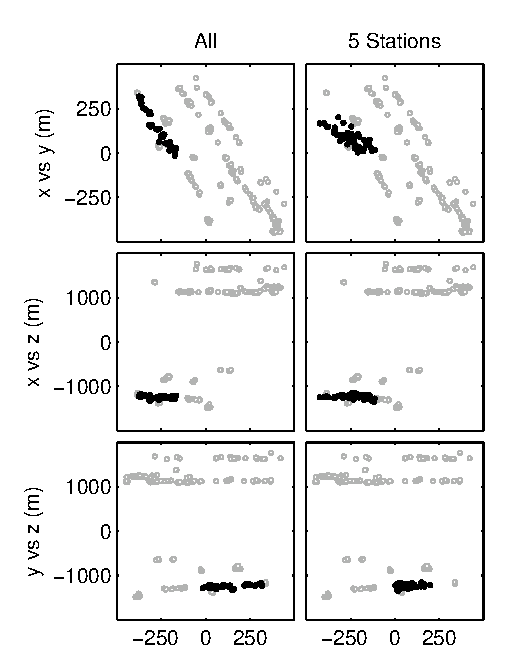
\includegraphics{diags/CalaverasLoc5_hypoDD_SVD.eps}
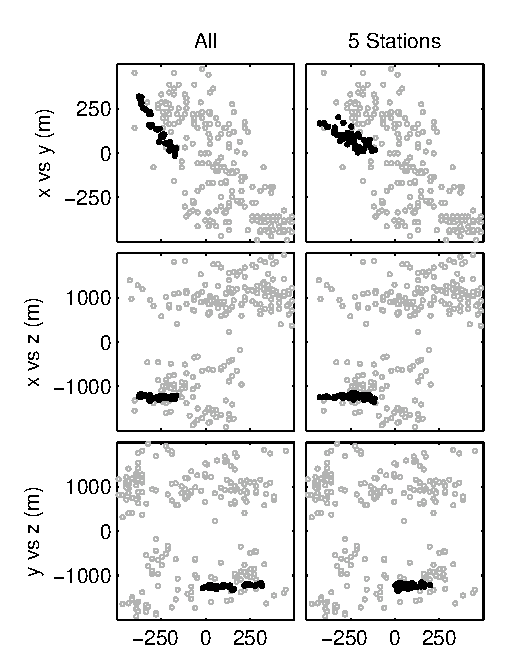
\includegraphics{Figure11_bw.eps}
\caption{Example 7 - Combined HypoDD (SVD) and CWI relative
locations using data form all stations (left) and 5 stations
(right). Axes as defined in Figure \ref{fig-69Calaverasevents_eg1}.} 
\label{fig-68Calaverasevents_ttandcoda1}
\end{figure}


%%=========================================================================

% Figure 12

\begin{figure}
%\noindent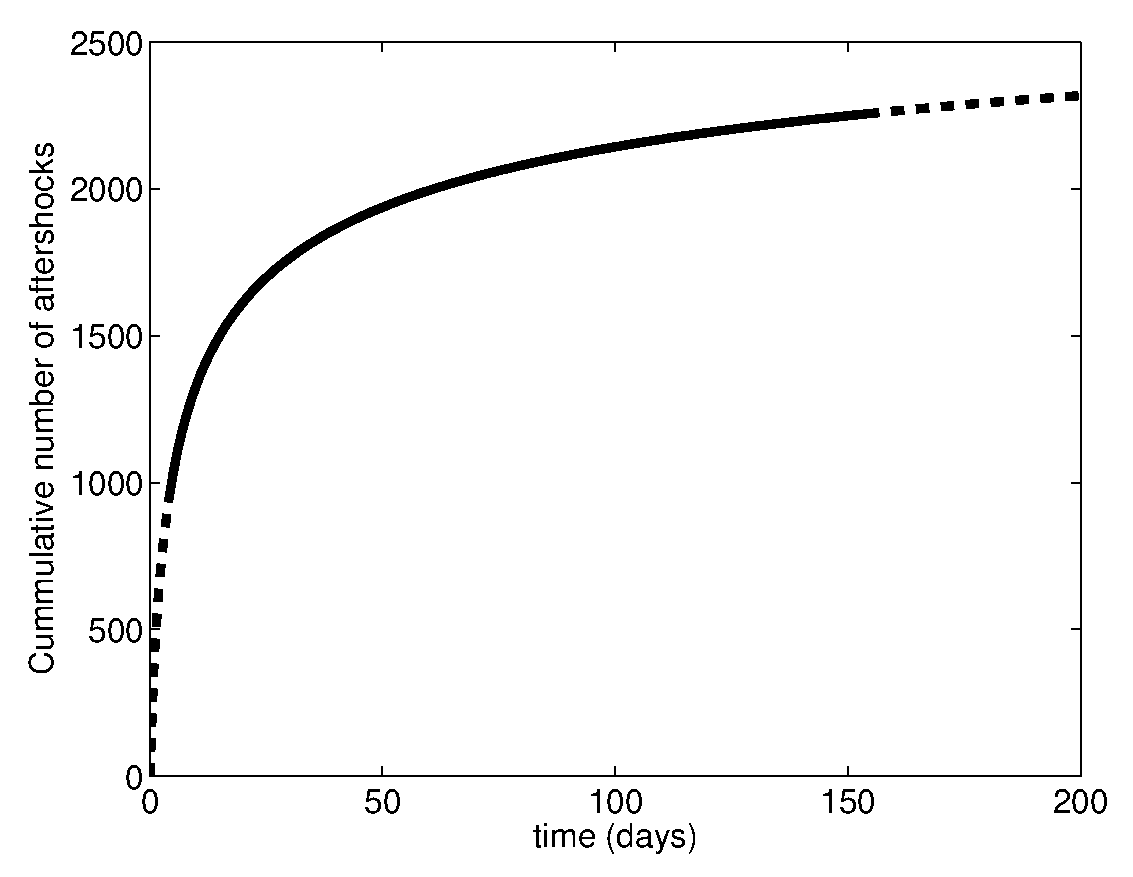
\includegraphics[width = 20pc]{diags/OmoriFigure.eps}
\noindent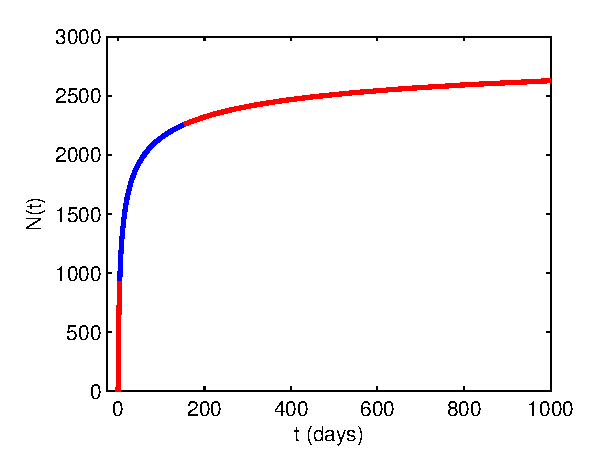
\includegraphics[width = 20pc]{Figure12_c.eps}
\caption{Modeled cumulative number of aftershocks for the
Hokkaido-Nansei-Oki, Japan $M_s=7.8$ earthquake of 12 July 1993
using equation (\ref{eq:CumOmori}). The leftmost, middle
and rightmost lines signify aftershocks occurring before, during
and after the deployment of a pseudo temporary array installed 4
days after the main shock and left for 150 days. A temporary
deployment of this kind will record roughly 50\% of the aftershocks
in the 1000 days following the mainshock. } \label{fig:Omorifigure}
\end{figure}

%%=========================================================================

% Figure 13

% This is the version using hypoDD with SVD
\begin{figure}
%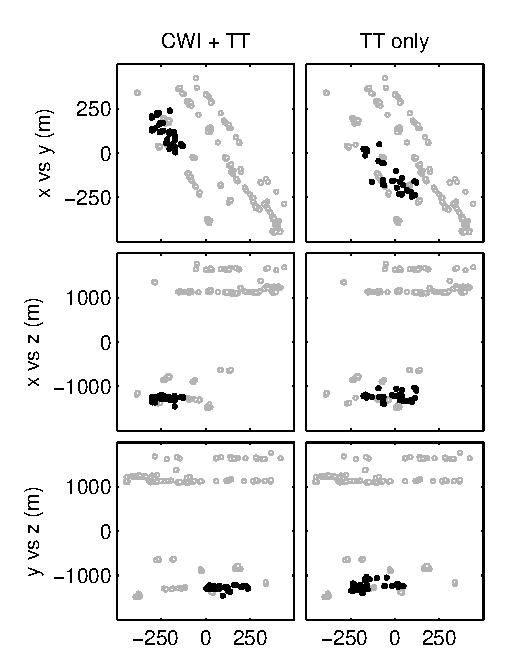
\includegraphics{diags/CalaverasLoc6_hypoDD_SVD.eps}
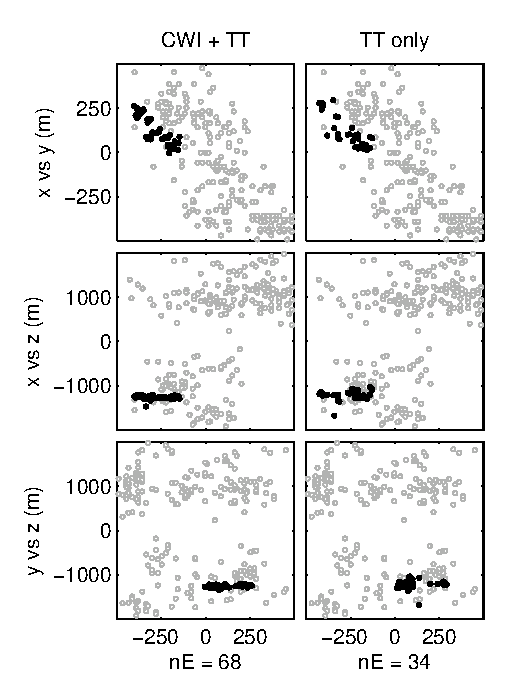
\includegraphics{Figure13_bw.eps}
\caption{Example 8 - Mimicking the deployment of a temporary network
by ignoring data from all but station CCO for 50\% (or 34) of the 68
events. Relative locations are shown for the combined CWI and arrival-time 
inversion (left) and the inversion with arrival-times only
(right). Only by combining the data is it possible to locate all 68
events. Furthermore, combining the data leads to a solution more
consistent with Figure \ref{fig-69Calaverasevents_eg1}. Axes as defined 
in Figure \ref{fig-69Calaverasevents_eg1}.}
\label{fig-68Calaverasevents_ttsubsetandcoda1}
\end{figure}
%%=========================================================================

\end{document}
